\section{Following the fixed failure-origin paths}
\label{sec:process}

\subsection{The fixed cohort, first-pass stopping, and exit}
\label{subsec:process-cohort}
We return to the high-confidence reconstruction defined in Sections~\ref{subsec:segment-rule} and~\ref{subsec:failure-cohort}. Its 367 edges form 262 full continuous segments. Selecting the 230 segments with an explicit failure at their origin gives the fixed cohort of 182 tasks. Selecting origins and stopping observation at first pass are separate operations; later records are never appended solely because they belong to the same task.

As defined in Section~\ref{sec:process-theory}, step 1 is the first eligible transition from the failing origin to another submitted candidate. Its outcome is the later candidate's recorded review decision. Each subsequent step is another such submitted-version transition. A path stops at its first recorded pass or at the end of the permitted chain, whichever comes first. The 230 paths contribute 329 observed steps in total. A row containing one such step and its outcome is called an \emph{eligible-step row}, traditionally a \emph{risk row}. ``At risk'' here means still eligible to record a \emph{first} pass.

There are two terminal outcomes. A total of 206 paths record a pass before the chain ends. The other 24 reach the chain boundary without such a pass. For this question, exit is an observed endpoint, not an unknown outcome silently assigned a failure label. It describes where this analytical path ends. It does not establish that the task was abandoned, that all future submissions would fail, or that an eventual pass elsewhere should be added to this path.

Changing the question changes the treatment of exits. If we asked how long the task would take to pass \emph{if the same mechanism continued indefinitely}, the post-exit outcomes would be unobserved. Calling those observations censored would not make the missing continuation known: additional assumptions would be needed to relate it to the observed paths. We do not estimate that hypothetical waiting time.

\subsection{Step counts, risk sets, and cumulative proportions}
\label{subsec:risk-counts}
At step 1 all 230 failure-origin paths are eligible. Of them, 167 pass, 18 end without a pass, and 45 continue to step 2:
\[
230=167+18+45.
\]
At step 2 only those 45 continuing paths remain. There are 29 passes, 4 exits, and 12 further continuations:
\[
45=29+4+12.
\]
The second denominator is 45 because we are asking about paths that reach step 2. It is not another sample of 230 paths, and it is not a comparison of all tasks before and after one extra revision. Table~\ref{tab:process-counts} shows the same accounting through the final observed step.

\begin{table}[htbp]
\centering
\caption{The fixed 230-path cohort. Each row partitions the paths observed at that step into pass, exit, or continuation.}
\label{tab:process-counts}
\small
\begin{tabular}{rrrrr}
\toprule
Step & Eligible & Pass & Exit & Continue \\
\midrule
1 & 230 & 167 & 18 & 45 \\
2 & 45 & 29 & 4 & 12 \\
3 & 12 & 1 & 0 & 11 \\
4 & 11 & 5 & 0 & 6 \\
5 & 6 & 2 & 1 & 3 \\
6 & 3 & 0 & 0 & 3 \\
7 & 3 & 0 & 0 & 3 \\
8 & 3 & 0 & 0 & 3 \\
9 & 3 & 0 & 0 & 3 \\
10 & 3 & 0 & 0 & 3 \\
11 & 3 & 1 & 0 & 2 \\
12 & 2 & 1 & 0 & 1 \\
13 & 1 & 0 & 0 & 1 \\
14 & 1 & 0 & 0 & 1 \\
15 & 1 & 0 & 0 & 1 \\
16 & 1 & 0 & 0 & 1 \\
17 & 1 & 0 & 1 & 0 \\
\midrule
Sum across steps & 329 & 206 & 24 & --- \\
\bottomrule
\end{tabular}
\end{table}

To write this bookkeeping once for all steps, let $n_j$ be the eligible count at step $j$, $d_j$ the passes at that step, and $c_j$ the exits after a nonpassing step. Then
\begin{equation}
 n_j=d_j+c_j+n_{j+1}.
 \label{eq:cohort-conservation}
\end{equation}
This is a counting identity, not a fitted model. The set of $n_j$ paths is the step-$j$ \emph{risk set}. Its decline is explained by the recorded pass and exit counts, without assuming a constant pass probability.

Two useful cumulative quantities keep the \emph{original} denominator 230:
\begin{align}
 F_P(j)&=\frac{d_1+\cdots+d_j}{230},
 &F_X(j)&=\frac{c_1+\cdots+c_j}{230}.
 \label{eq:finite-incidences}
\end{align}
$F_P(j)$ is the fraction of original paths that have passed by step $j$; $F_X(j)$ is the fraction that have exited without a pass by that step. The letters $P$ and $X$ stand for pass and exit. These are cumulative proportions, also called cumulative incidences. The remaining fraction is $n_{j+1}/230$, so the three fractions add to 1. At the last observed step,
\[
 F_P(17)=206/230=89.57\%,\qquad
 F_X(17)=24/230=10.43\%.
\]
Because exit is one of the two recorded terminal outcomes, calculating these finite-path proportions requires no assumption that exits are independent of future success.

Let a path's \emph{observed length} be its number of eligible transitions up to pass or exit. Adding those lengths gives 329. Their mean is therefore $329/230=1.4304$ transitions per path. A short path can end either in a pass or in an exit, so this is not the mean number of edits required for eventual success.

\subsection{First-step and later-step proportions have different composition}
\label{subsec:first-later}
All first steps together give $167/230=72.61\%$ recorded passes. All steps with index 2 or greater together give $39/99=39.39\%$. The denominator 99 is the sum of the later eligible counts in Table~\ref{tab:process-counts}, not 99 distinct paths or 99 independent tasks. A long path contributes several later rows. The difference ``later minus first'' is
\[
100\left(\frac{39}{99}-\frac{167}{230}\right)=-33.21
\quad\text{percentage points}.
\]
This is a description of two groups of observed rows. It is not the change that would occur if each of the same tasks were forced to receive exactly one more revision.

To show how these summaries vary under a reference sampling model, we resampled 182 entire tasks, with replacement, 20,000 times using the fixed seed 20260906. Whenever a task was selected, all its original paths and eligible rows were retained together. Each replicate recomputed the relevant ratio from pooled counts. The 2.5th and 97.5th percentiles of those results form the 95\% task-cluster reference intervals in Table~\ref{tab:process-estimates}. This preserves dependence within a task during resampling. It does not establish independence between tasks or adjust the observed history for selection. The interpretation of these reference intervals is explained in Section~\ref{subsec:cluster-resampling}.

\begin{table}[htbp]
\centering
\caption{Observed summaries and 95\% whole-task percentile reference intervals. Percentage-point differences use subtraction of proportions; observed length is measured in submitted-version transitions.}
\label{tab:process-estimates}
\small
\begin{tabularx}{\linewidth}{Yrr}
\toprule
Quantity & Estimate & Reference interval \\
\midrule
First-step pass proportion & $72.61\%$ & $[66.40,78.60]\%$ \\
Later-step pass proportion & $39.39\%$ & $[24.84,65.71]\%$ \\
Later minus first, percentage points & $-33.21$ & $[-48.39,-7.49]$ \\
Pass before fixed-path exit & $89.57\%$ & $[85.40,93.53]\%$ \\
Mean observed length to pass or exit & $1.4304$ & $[1.2271,1.6955]$ \\
\bottomrule
\end{tabularx}
\end{table}

These are ratios of pooled task totals, not means that give every task equal weight irrespective of its number of paths or rows. They therefore differ in weighting from the task-equal edge analysis in Section~\ref{sec:statistics}. The later-step interval is wide because the later rows are limited and unevenly distributed across tasks. For the already enumerated archive, the displayed proportions themselves are exact descriptions up to rounding; the intervals concern a hypothetical repetition under independent, exchangeable tasks with the same record-selection mechanism. Those assumptions have not been established by this archive.

\begin{figure}[htbp]
\centering
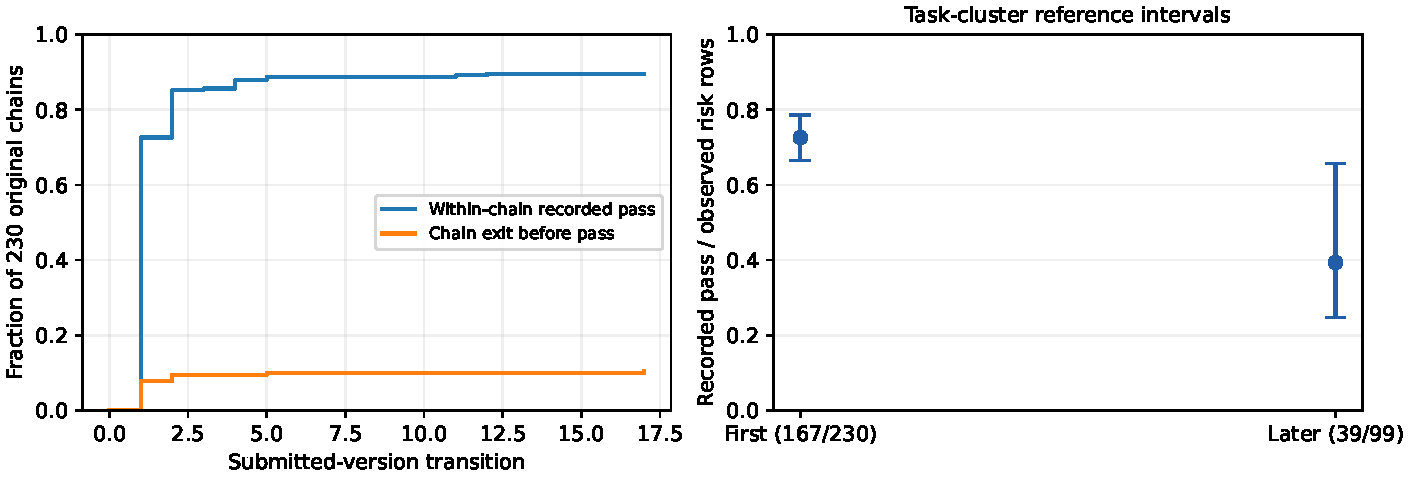
\includegraphics[width=\linewidth]{../figures/process_profile.pdf}
\caption{The same process information in graphical form. Left: cumulative pass and exit proportions among the original 230 paths. Right: first and later observed-step proportions with whole-task percentile reference intervals. The figure describes recorded paths and does not estimate the effect of another edit.}
\label{fig:process}
\end{figure}

\subsection{The two-group logit model and its coefficients}
\label{subsec:two-group}
The process model compares recorded-pass means in the first-step and later-step row groups. On the logit scale,


\[
\operatorname{logit}(r)=\log\left(\frac{r}{1-r}\right),
\qquad
r=\frac{\exp(u)}{1+\exp(u)}\quad\text{when }u=\operatorname{logit}(r).
\]
The outcome concerns observed eligible rows, and the two groups can contain different mixtures of tasks.

Index a task by $s$, a path within that task by $e$, and a step within that path by $j$. For an observed eligible row, define $Y_{sej}=1$ for a recorded pass and $Y_{sej}=0$ otherwise. Let $L_j$ be the later-step indicator: it is 0 when $j=1$ and 1 when $j\ge2$. Finally, let $\mu_{sej}$ denote the mean of this binary outcome within the indicated observed-row group. The fitted equation is
\begin{equation}
 \operatorname{logit}(\mu_{sej})=\alpha+\beta L_j.
 \label{eq:process-two-group-model}
\end{equation}
$\alpha$ is the first-step log-odds. The coefficient $\beta$ is the amount added to those log-odds for a later step. Thus $\exp(\beta)$ is the later-to-first odds ratio. There are only two fitted group means; the equation does not give each task its own baseline or control for task difficulty.

The analysis fits this equation using \emph{generalized estimating equations}, or GEE, for binary outcomes, with a working-independence calculation and a robust task-cluster covariance.\cite{statsmodelsgee} In this simple two-group case the fitted means are exactly the two empirical proportions. The coefficients can therefore be checked directly from the group counts:
\begin{align*}
 \widehat\alpha&=\log(167/63)=0.974859,\\
 \widehat\beta&=\log(39/60)-\log(167/63)=-1.405642.
\end{align*}
There are 63 nonpassing first rows and 60 nonpassing later rows. Substituting $L_j=0$ into the inverse-logit formula recovers $0.726087$; substituting $L_j=1$ recovers $0.393939$. Exponentiating the difference gives
\[
\exp(\widehat\beta)=\frac{39/60}{167/63}=0.2452.
\]
This is the odds ratio for the two observed-row groups, not an estimate of a revision's causal effect.

\subsection{Task-cluster covariance and the reference test}
\label{subsec:robust-covariance}
Several rows from the same task can share candidate history, requirements, and review circumstances. Treating all 329 rows as unrelated observations would disregard that structure. The covariance is clustered by task to account for within-task dependence; the two fitted proportions remain unchanged.

``Working independence'' names a computational choice for the fit, not a finding that successive submissions are actually independent. The correction also does not make different tasks independent: shared dependencies, models, rules, or collection batches can connect them. Nor does clustering remove task difficulty or the selection that lets a path reach later steps.

The robust standard error for $\widehat\beta$ is $0.413295$. The approximate 95\% Wald interval uses a normal reference and the task-cluster covariance. On the log-odds scale,
\[
-1.405642\ \pm\ 1.96(0.413295)
\approx[-2.215685,-0.595599].
\]
Exponentiating its endpoints gives the odds-ratio interval $[0.1091,0.5512]$. Dividing the coefficient by its standard error gives approximately $-3.4011$; comparison with a standard normal reference distribution yields the nominal two-sided value $p=0.0006712$. Here the null hypothesis is $\beta=0$, equivalently equal fitted first and later means or odds ratio 1. As with the tests in Section~\ref{sec:statistics}, this is a conditional reference calculation, with no test of semantic correctness.

The covariance was independently reconstructed from the task contributions. Its maximum absolute difference from the software calculation was $2.5\times10^{-16}$, and an independent verification also reproduced the task-level resampling results. This checks the computation against the stated inputs and formula. It does not validate the row-selection mechanism or establish a causal explanation for the association.

For comparison, forcing one common mean gives the pooled rate $206/329=0.626140$. The independent-Bernoulli working model for $d$ passes in $n$ rows has likelihood
\[
 \mathcal L(r)=r^d(1-r)^{n-d},\qquad 0<r<1.
\]
For the \emph{working log-likelihood} $\ell(r)=\log\mathcal L(r)$,
\[
 \ell(r)=d\log r+(n-d)\log(1-r),\qquad
 \ell'(r)=\frac d r-\frac{n-d}{1-r}.
\]
Setting this derivative to zero gives $d(1-r)=(n-d)r$, hence $r=d/n$. When both outcomes occur, the second derivative is negative, so this is the maximum. Substituting the observed $d=206,n=329$ yields the pooled rate above.

This is an \emph{independent-Bernoulli working likelihood}, not a full joint likelihood for an unspecified dependent task process. Maximizing this convenient function does not establish the independence it assumes. Moreover, the restriction $\beta=0$ compares only two observed-row group means. The constant conditional probability in Proposition~\ref{prop:stopping} demands equality after every eligible past history, a substantially stronger statement. This two-group test neither verifies nor exhaustively tests that stronger model. In particular, it does not show that making another revision causes a lower chance of success.

\subsection{Why selecting tasks with later observations changes the first-step group}
\label{subsec:later-selection}
Only 39 of the 182 tasks contribute later-step rows. If we select those tasks after examining the whole history, their first-step rows contain 12 passes among 61 rows, or $19.67\%$. The later-row rate of $39.39\%$ now looks higher than the selected first-row rate, whereas it was lower than the full first-row rate of $72.61\%$. The arithmetic is correct, but the populations changed.

The reason becomes clear when the 61 first rows are separated. Forty-five belong to paths that actually continued. Every one of those first steps must be nonpassing under our first-pass stopping rule, so their count is necessarily $0/45$. The remaining 16 are first rows of other paths belonging to those same 39 tasks; 12 of these pass. Therefore $61=45+16$ and $12=0+12$. Selecting tasks because they have later observations deliberately retains many first steps that had to fail in order to continue.

This selection uses future information relative to step 1. It is not a balanced comparison of the same tasks under two assigned numbers of revisions. The reversal does not by itself identify an improvement mechanism, a difficulty mechanism, or a causal effect. Naming it after a statistical paradox would not replace the needed explanation of the denominators.

As a limited influence check, removing one task at a time gives later-minus-first differences between $-36.07$ and $-23.57$ percentage points, and odds ratios between $0.2156$ and $0.3593$. No single-task removal reverses this pooled association, but that does not settle dependence across tasks or selection of the archive. Adding medium-confidence edges can reconnect paths and change the failure-origin cohort itself. Such a change answers a different-cohort question; we retain the original high-confidence paths here.

The process results thus make a bounded claim: they describe when recorded passes and exits occur within a specified historical reconstruction, and quantify the association of recorded outcomes with observed process position. They do not estimate the causal value of another edit, the probability of mathematical truth, or the waiting time under an unobserved continuation policy. The accompanying frozen inputs and scripts make those particular calculations reproducible without adding new review experiments.
